\documentclass{article}
\usepackage{graphicx} % Required for inserting images
\usepackage{tabularx}
\usepackage{float}
\usepackage{blindtext}
\usepackage{hyperref}
\usepackage{booktabs}
\usepackage[bottom]{footmisc}  % Place footnotes at the bottom of the page

% Customize footnote numbering style
\renewcommand{\thefootnote}{\arabic{footnote}}  % Use lowercase letters for numbering

\title{Datos y Metodología Paper}
\author{}
\date{Septiembre 2023}

\begin{document}

\maketitle

\section{Data}
Since the purpose of this paper is to study the effects of natural disasters on the mean and variance 
of financial series in emerging economies, we retrieved data from several sources. Firstly, we 
downloaded the 5-year sovereign Credit Default Swap $(CDS)$ daily series for all the countries of 
interest: Brazil, Chile, China, Colombia, Indonesia, South Korea, Malaysia, Mexico, Peru, South Africa, and Turkey. 
The sample we were able to obtain starts on October 10, 2004, and it ends on August 10, 2022. In Table \ref{table:CDS}
 we present the descriptive statistics of the first difference of all the CDS series. \\
\begin{table}[H]
\centering
\small
\begin{tabular}{rrrrrrr}
  \hline
Country & Minimum & Maximum & Mean & Std. Dev. & Skewness & Kurtosis \\ 
  \hline
Brazil & -124.91 & 186.53 & -0.03 & 8.45 & 2.01 & 81.53 \\ 
  Chile & -64.27 & 63.11 & 0.02 & 3.71 & 0.66 & 67.48 \\ 
  China & -58.91 & 67.47 & 0.01 & 3.52 & 0.63 & 73.61 \\ 
  Colombia & -126.52 & 180.59 & -0.02 & 8.20 & 1.38 & 83.91 \\ 
  Indonesia & -223.81 & 324.52 & -0.06 & 13.30 & 3.12 & 170.85 \\ 
  South Korea & -168.55 & 133.28 & 0.00 & 5.72 & -2.92 & 266.79 \\ 
  Malaysia & -101.34 & 119.40 & 0.01 & 5.22 & 1.71 & 128.90 \\ 
  Mexico & -132.96 & 197.20 & 0.01 & 7.31 & 3.82 & 168.49 \\ 
  Peru & -126.10 & 161.39 & -0.04 & 6.72 & 1.82 & 120.92 \\ 
  South Africa & -82.36 & 146.45 & 0.03 & 7.99 & 2.25 & 58.39 \\ 
  Turkey & -131.91 & 166.47 & 0.08 & 10.72 & 1.57 & 48.01 \\ 
  Moving Average & -11.46 & 20.19 & 0.01 & 1.33 & 3.17 & 50.01 \\ 
   \hline
\end{tabular}
\caption{Descriptive Statistics CDS spreads}
\label{table:CDS}
\end{table}
We also aimed to assess the impact of natural disasters on the major stock indices of various countries. 
We utilized the following indices: Bovespa for Brazil, S\&P CLXIPSA for Chile, ChinaA50 for China, 
COLCAP for Colombia, JSX for Indonesia, KOSPI for South Korea, KLCI for Malaysia, S\&P BMVIPC for 
Mexico, IGBVL for Peru, South Africa Top 40 for South Africa, and BIST100 for Turkey. Table 
\ref{table:stock} presents the descriptive statistics of the returns for all these stock index 
series, covering the same sample period as the CDS data, from October 10, 2004, to August 10, 2022. \\

\begin{table}[H]
\centering
\small
\begin{tabular}{rrrrrrr}
  \hline
 Stock Index & Min. & Max. & Mean & Std. Dev. & Skewness & Kurtosis \\ 
  \hline
BIST100 & -11.06 & 12.13 & 0.06 & 1.59 & -0.53 & 7.53 \\ 
  Bovespa & -15.99 & 13.68 & 0.03 & 1.68 & -0.43 & 12.70 \\ 
  ChinaA50 & -9.86 & 9.20 & 0.02 & 1.61 & -0.24 & 7.57 \\ 
  JSX & -10.95 & 7.62 & 0.05 & 1.22 & -0.62 & 10.39 \\ 
  KOSPI & -11.17 & 11.28 & 0.02 & 1.20 & -0.47 & 12.30 \\ 
  S\&P BMVIPC & -7.27 & 10.44 & 0.03 & 1.17 & -0.01 & 9.66 \\ 
  S\&P CLXIPSA & -15.22 & 11.80 & 0.02 & 1.12 & -0.80 & 23.81 \\ 
  SouthAfricaTop40 & -10.45 & 9.11 & 0.04 & 1.29 & -0.20 & 8.76 \\ 
  IGBVL & -117.48 & 230.26 & 0.04 & 4.40 & 23.49 & 1842.97 \\ 
  KLCI & -9.98 & 6.63 & 0.01 & 0.72 & -0.88 & 17.32 \\ 
  COLCAP & -16.29 & 14.69 & 0.03 & 1.25 & -0.80 & 26.72 \\ 
  Moving Average & -1.81 & 0.86 & 0.03 & 0.22 & -1.59 & 12.39 \\ 
   \hline
\end{tabular}
\caption{Descriptive Statistics Stock Indexes Returns}
\label{table:stock}
\end{table}

In light of the diverse range of countries represented in our sample, we have opted to employ the internationally recognized Emergency Events Database (EM-DAT) published by the Centre for Research on the Epidemiology of Disasters (CRED)\footnote{This database can be 
accesed in the next link \href{https://www.emdat.be/}{https://www.emdat.be/}}. Our data collection focused on cataloging natural disasters occurring within the time frame spanning from October 10, 2004, to August 10, 2022, within our selected countries of interest. While the EM-DAT initially comprised 1400 natural disasters, we excluded three cases due to a lack of information regarding their respective start months. Consequently, we obtained a dataset encompassing 1397 disasters, classified into five distinct and mutually exclusive categories: Biological, Climatological, Geophysical, Hydrological, and Meteorological. \\
According to the Peril Classification and Hazard Glossary, as defined by the Integrated Research on Disaster Risk (IDRD), geophysical disasters originate from solid earth processes, hydrological disasters stem from occurrences, movements, and distributions of surface and subsurface freshwater and saltwater, meteorological disasters result from \textbf{short-lived} extreme weather conditions, climatological disasters arise from \textbf{long-lived} atmospheric processes, and biological disasters are triggered by exposure to living organisms or their toxic substances, as well as diseases they may carry. In Table \ref{tab:disasters} we provide a breakdown of the disasters corresponding to each disaster type.\\
Meanwhile, Table \ref{tab:disaster_type} presents the count and the proportion of each type and subtype of disaster within our sample. Notably, our analysis reveals that the most prevalent types of disasters in our sample are hydrological, meteorological, and geophysical. Conversely, the most frequent subtypes of disasters are floods, accounting for $46.81\%$ of the sample, storms at $20.26\%$, and earthquakes at $13.96\%$ of the total sample.

\begin{table}[H]
    \centering
    \footnotesize
    \begin{tabular}{p{2.5cm}p{2.5cm}p{2.5cm}p{2.5cm}}
    \toprule 
       Disaster Sub-Group  & Disaster Type & Disaster Sub-Type & Disaster Sub-sub Type  \\
       \midrule
        Geophysical & Earthquake & Ground Movement &\\
        & & Tsunami & \\\cmidrule{2-4}
        & Volcanic Activity & Ash fall& \\
        && Lahar&\\
        && Pyroclastic Flow &\\
        && Lava Flow &\\ \cmidrule{2-4}
        & Mass movement & &\\
    \midrule
    Meteorological & Storm & Tropical Storm &\\
    & & Extra-tropical Storm& \\
    && Convective Storm & Derecho \\
    && & Hail \\
    && & Lightning/Thunderstorm \\
    && & Rain \\
    && & Tornado \\
    && & Sand-dust Storm \\
    && & Winter Storm/Blizzard \\
    && & Storm/Surge \\
    && & Wind \\
    && & Severe storm \\ \cmidrule{2-4}
    & Extreme temperature & Cold wave &\\
    && Heat wave & \\
    && Severe wind conditions & Snow-ice \\
    &&& Frost/Freeze\\ \cmidrule{2-4}
    & Fog && \\
    \midrule
    Hydrological&Flood&Coastal flood&\\
    &&Riverine flood&\\
    &&Flash flood&\\
    &&Ice jam flood&\\ \cmidrule{2-4}
    & Landslinde & Avalanche (snow,debris, mudflow, rock fall) &\\
    \cmidrule{2-4}
    & Wave action & Rogue wave &\\
    && Seiche &\\ 
    \midrule
    Climatological & Drought & Drought &\\ \cmidrule{2-4}
    & Glacial Lake Outburst && \\ \cmidrule{2-4}
    & Wildfire & Forest fires & \\
    && Land fire: brush, bush, pasture &\\
    \midrule
    Biological & Epidemic & Viral diseases &\\
    && Bacterial diseases & \\
    && Parasitic diseases & \\
    && Fungal diseases & \\
    && Prion diseases & \\ \cmidrule{2-4}
    & Insect infestation & Locust & \\
    & & Grasshopper & \\ \cmidrule{2-4}
    & Animal accident \\
    \bottomrule
    \end{tabular}
    \caption{List of disasters for each type of disaster}
    \label{tab:disasters}
\end{table}

\begin{table}[H]
    \centering
    \begin{tabular}{llll}
       Disaster Type & Disaster Subtype & Count & Proportion \\
       \toprule
        Biological & Epidemic & 20 & 1.43\%\\
        & \textbf{Subtotal} & \textbf{20} & \textbf{1.43\%} \\ \cmidrule{2-4}
        Climatological & Drought& 33 & 2.36\% \\
        & Wildfire & 28 & 2.00\% \\ 
        & \textbf{Subtotal} & \textbf{61} & \textbf{4.36\%} \\ \cmidrule{2-4}
        Geophysical & Earthquake & 195 & 13.96\% \\
        & Volcanic Activity & 35 & 2.51\% \\
        & Mass Movement & 4 & 0.29\% \\
        & \textbf{Subtotal} & \textbf{234} & \textbf{16.76\%} \\ \cmidrule{2-4}
        Hydrological & Flood& 654 & 46.81\% \\
        & Landslide & 115 & 8.23\% \\ 
        & \textbf{Subtotal} & \textbf{769} & \textbf{55.04\%} \\ \cmidrule{2-4}
        Meteorological & Storm& 283 & 20.26\% \\
        & Extreme temperature & 30 & 2.15\% \\ 
        & \textbf{Subtotal} & \textbf{313} & \textbf{22.41\%} \\ \cmidrule{2-4}
        Total & & 1397 & 100\% \\
        \bottomrule
    \end{tabular}
    \caption{Count and proportion of each disaster type}
    \label{tab:disaster_type}
\end{table}
Another method of representing the natural disasters
in our dataset is through the use of maps. Figure 
\ref{fig:climatological} illustrates the number of 
climatological disasters by country, Figure 
\ref{fig:geophysical} presents the count of 
geophysical disasters, Figure \ref{fig:hydrological} 
provides data on hydrological disasters, Figure 
\ref{fig:meteorological} showcases meteorological 
disasters, and Figure \ref{fig:todos} offers a 
comprehensive overview of all disasters in the 
sample.

\begin{figure}[H]
    \centering
    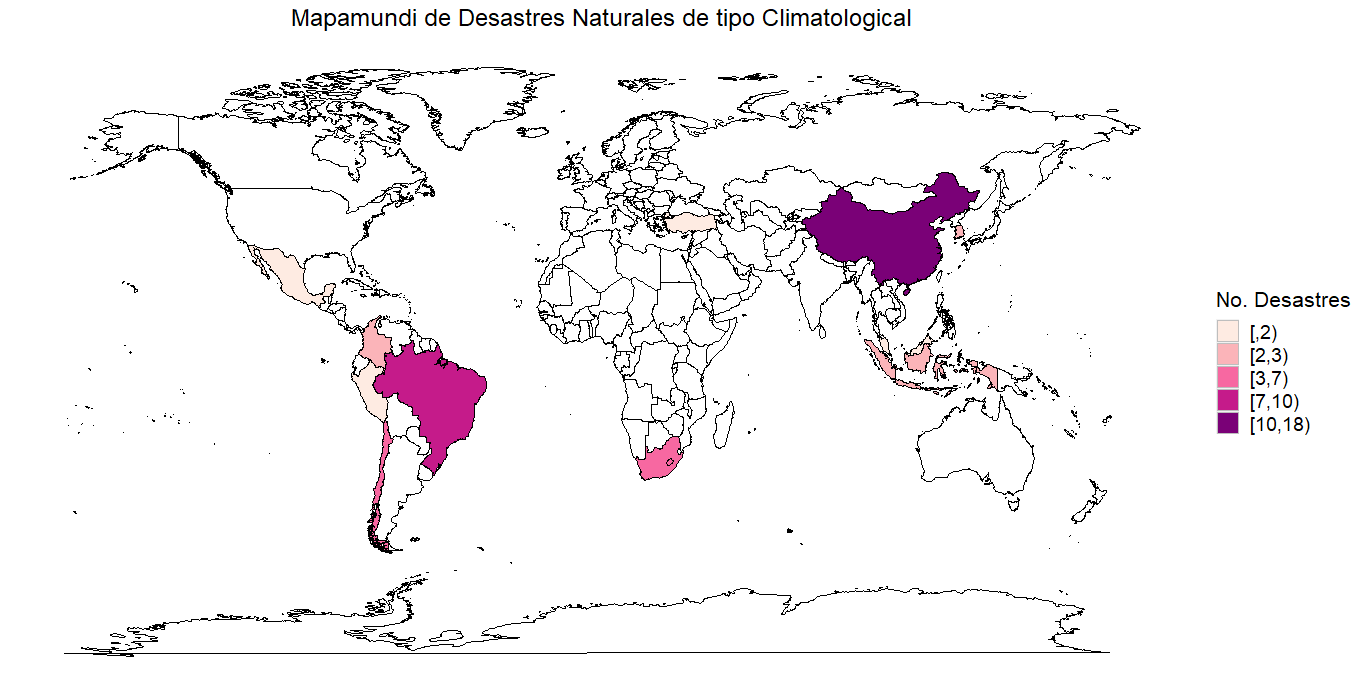
\includegraphics[width=\textwidth]{Imagenes/climatological.png}
    \caption{Frequency of climatological disasters.}
    \label{fig:climatological}
\end{figure}
\begin{figure}[H]
    \centering
    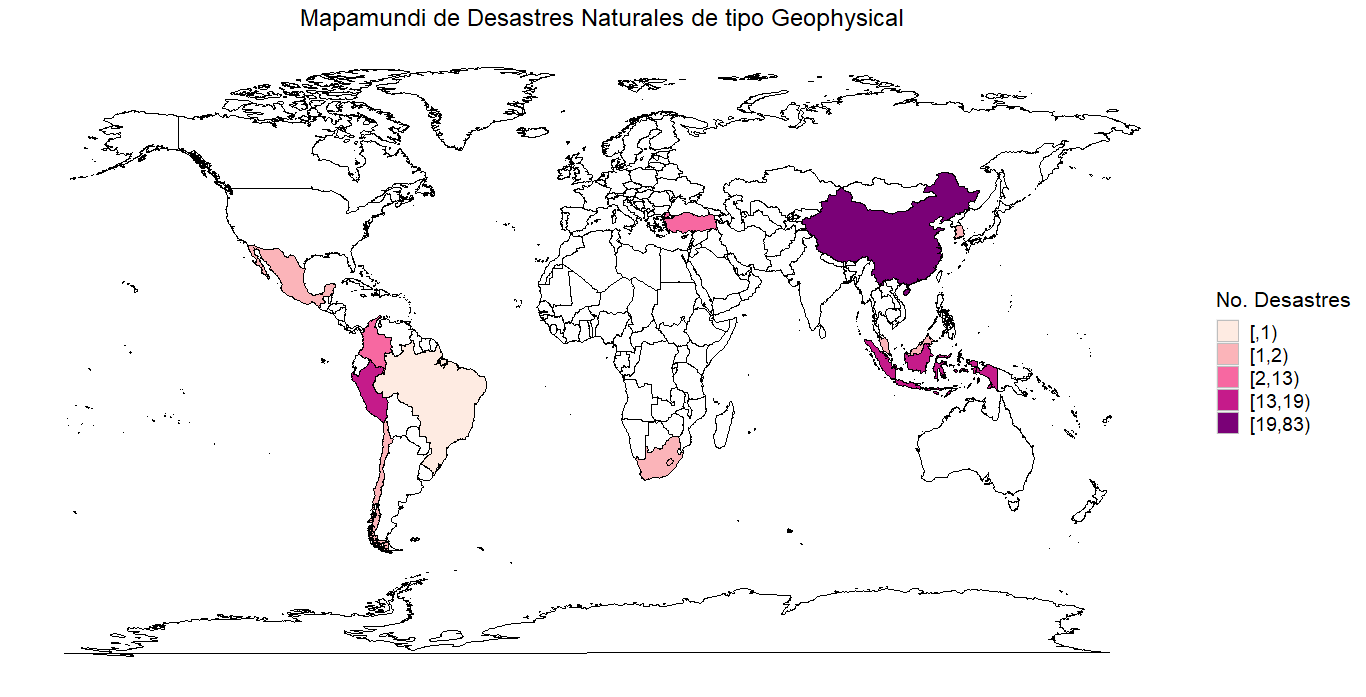
\includegraphics[width=\textwidth]{Imagenes/geophyisical.png}
    \caption{Frequency of geophysical disasters.}
    \label{fig:geophysical}
\end{figure}
\begin{figure}[H]
    \centering
    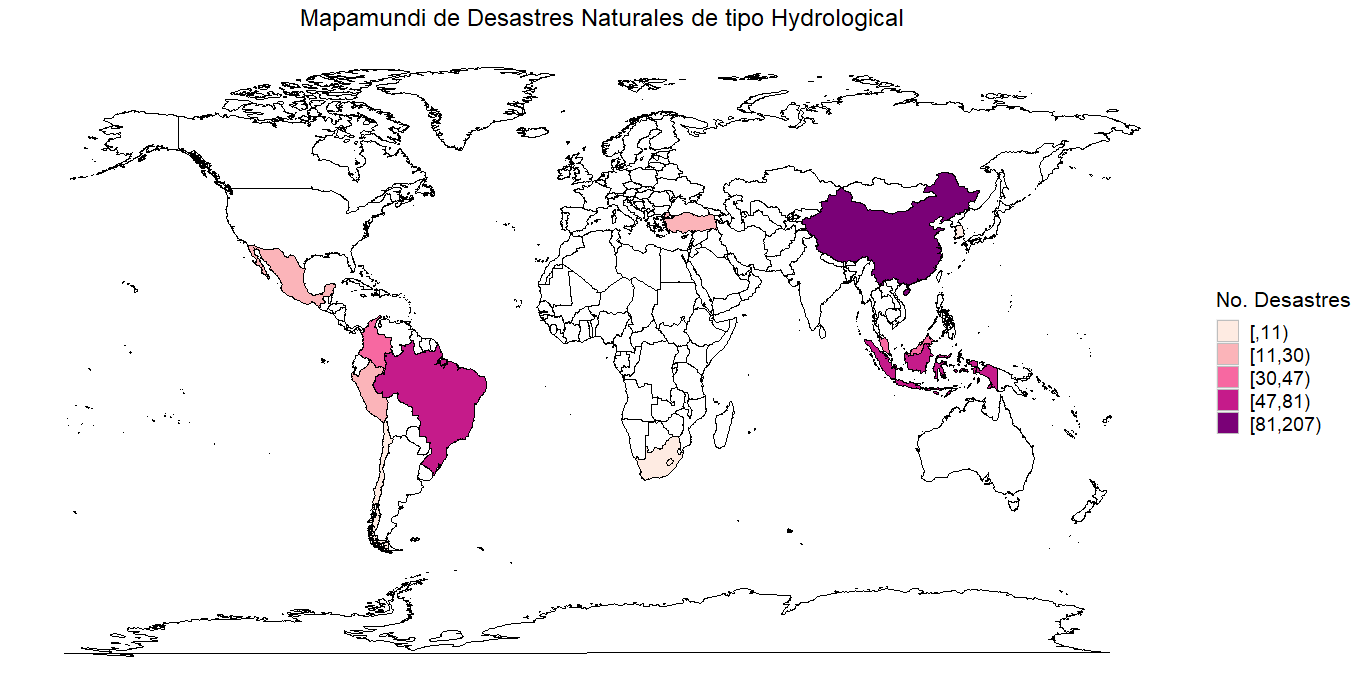
\includegraphics[width=\textwidth]{Imagenes/Hydrological.png}
    \caption{Frequency of hydrological disasters.}
    \label{fig:hydrological}
\end{figure}
\begin{figure}[H]
    \centering
    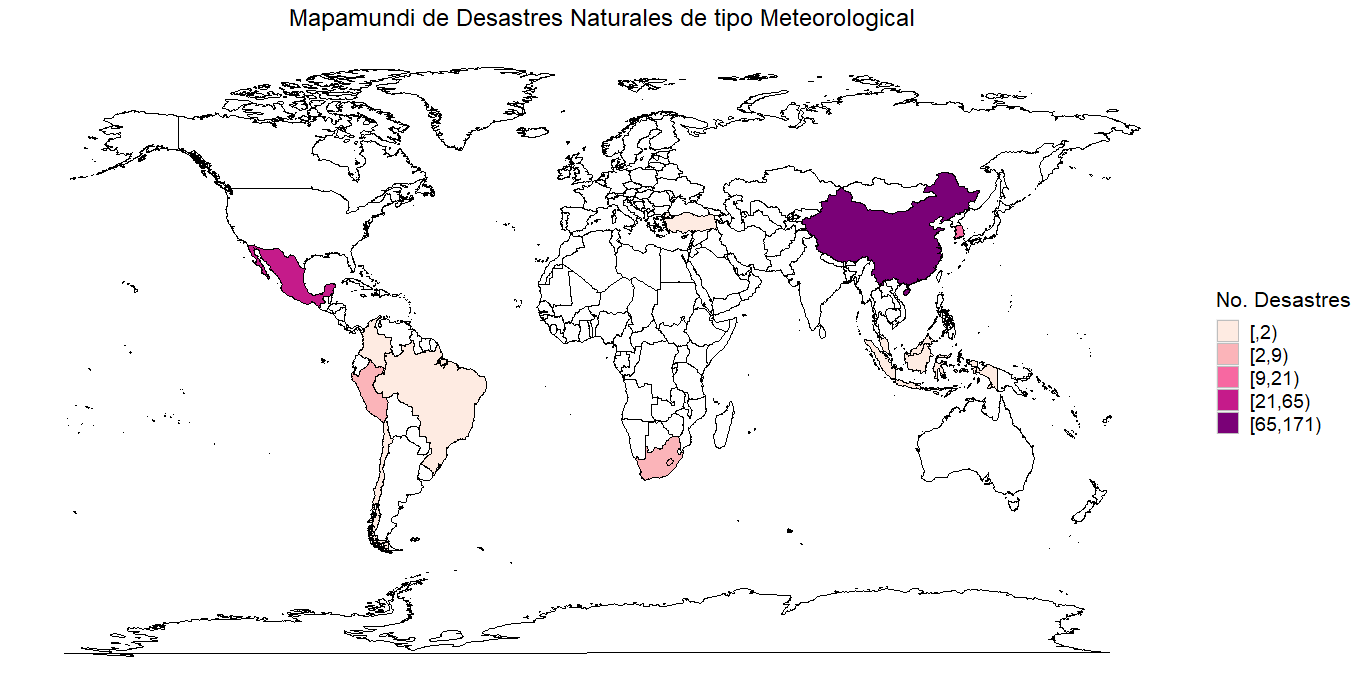
\includegraphics[width=\textwidth]{Imagenes/Meteorological.png}
    \caption{Frequency of meteorological disasters.}
    \label{fig:meteorological}
\end{figure}
\begin{figure}[H]
    \centering
    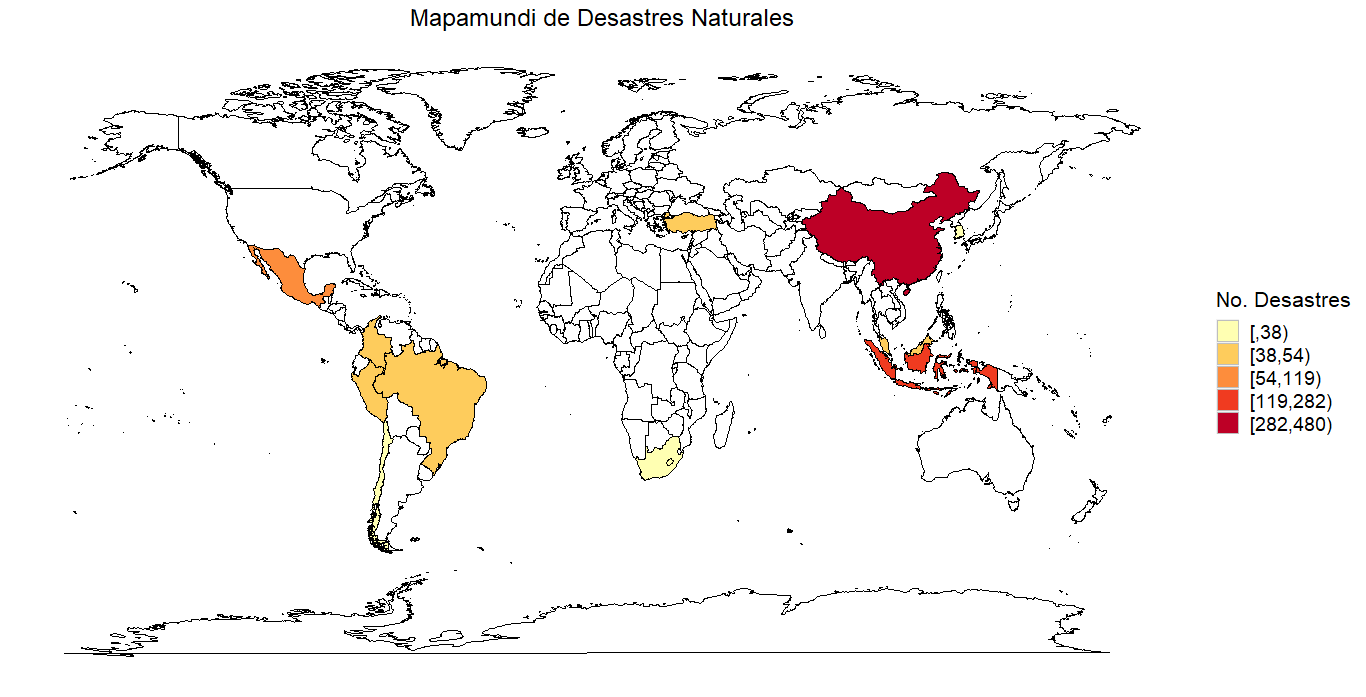
\includegraphics[width=\textwidth]{Imagenes/Todos.png}
    \caption{Frequency of natural disasters.}
    \label{fig:todos}
\end{figure}
As the event study method's effectiveness hinges on the precise identification of the event's commencement date, we opted to exclude the outcomes pertaining to disasters lacking information about their initiation date, accounting for 6.37\% of the data set. By doing this, the number of biological disasters is reduced from 20 to 5, so we decided to drop this category from our analysis. \\
Conversely, in line with Cavallo, Becerra, and Acevedo\footnote{The Impact of Natural Disasters on Economic Growth}, we chose to eliminate the climatological category from our analysis. This decision was driven by the fact that these disasters tend to be less fatal and have considerably longer durations compared to other types of events.\\
According to the event study methodology, there is an estimation window, where we estimated the market model to calculate the expected returns after the disaster, and the event window, where we will test the abnormal returns due to the disaster. Subsequently, any disasters failing to meet the criteria of either window are excluded from the analysis. \\
Lastly, we applied a window to reduce the overlap of the estimation windows, since there were events that started roughly on the same date.This entailed selecting a defined window, such as 50 days, to ensure that within each 50-day period and for each country, only a single event was considered. The selection criteria for this event was based on the one with the highest number of people affected by the disaster.

\end{document}
